\documentclass[a4paper,10pt]{article}
%\documentclass{svjour3}
\usepackage{a4wide}
\usepackage[utf8]{inputenc}
\usepackage[T1]{fontenc}

%\usepackage{tcolorbox}
\usepackage{subcaption}
\usepackage{amsmath,amssymb}
\usepackage{amsthm}
%\usepackage{calrsfs} % nice cal fonts
\usepackage{enumerate} 
%\usepackage[toc,page]{appendix}

%\usepackage[auth-sc]{authblk}
\usepackage{authblk}
\renewcommand\Affilfont{\normalfont\small}

\usepackage[round]{natbib}
\bibpunct[, ]{(}{)}{;}{a}{}{,}
\let\bibfont\relax
\def\bibfont{\fontsize{8}{10}\selectfont}
\setlength{\bibsep}{0pt}

\usepackage[svgnames]{xcolor}
\usepackage[pdftex]{hyperref}
\hypersetup{
    colorlinks=true,
    colorlinks,
    linkcolor=Navy,
    citecolor=Navy,
    urlcolor=Navy
}
%\definecolor{highlightNEW}{named}{Navy} %To get all equation in black:
\definecolor{highlightNEW}{named}{black}

\usepackage{graphicx}
\graphicspath{{fig/}}
\usepackage{epstopdf}
\usepackage{booktabs}
\usepackage{multirow}

% custom macros and definitions
\newtheorem{theorem}{Theorem}[section] 
%%\newtheorem{acknowledgement}[theorem]{Acknowledgement} 
%%\newtheorem{algorithm}[theorem]{Algorithm} 
%%\newtheorem{axiom}[theorem]{Axiom} 
%%\newtheorem{case}[theorem]{Case} 
%%\newtheorem{claim}[theorem]{Claim} 
%%\newtheorem{conclusion}[theorem]{Conclusion} 
%%\newtheorem{condition}[theorem]{Condition} 
%%\newtheorem{conjecture}[theorem]{Conjecture}
\newtheorem{definition}[theorem]{Definition}
\newtheorem{corollary}[theorem]{Corollary} 
%%\newtheorem{criterion}[theorem]{Criterion} 
%%\newtheorem{defi}[theorem]{Definition} 
\newtheorem{example}[theorem]{Example} 
%%\newtheorem{exercise}[theorem]{Exercise} 
%%\newtheorem{hypothesis}[theorem]{Hypothesis} 
\newtheorem{lemma}[theorem]{Lemma} 
%%\newtheorem{notation}[theorem]{Notation} 
%%\newtheorem{problem}[theorem]{Problem} 
\newtheorem{proposition}[theorem]{Proposition} 
%%\newtheorem{question}[theorem]{Question} 
\newtheorem{remark}[theorem]{Remark} 
%%\newtheorem{solution}[theorem]{Solution} 
%%\newtheorem{summary}[theorem]{Summary} 
%%\newtheorem{Rem}[theorem]{Remark}

\newcommand{\TODO}[1]{\textbf{\color{red}TODO: {#1}}\PackageWarning{TODO:}{#1!}}
\newcommand{\doi}[1]{DOI~\href{\detokenize{http://dx.doi.org/#1}}{\detokenize{#1}}}

\renewcommand{\d}{\,\mathrm{d}}
\newcommand{\e}{\mathrm{e}}
\newcommand{\E}{\mathbb{E}}
\newcommand{\F}{\mathcal{F}}
\renewcommand{\H}{\mathcal{H}}
\newcommand{\K}{\mathfrak{K}}
\newcommand{\N}{\mathbb{N}}
\renewcommand{\P}{\mathbb{P}}
\newcommand{\R}{\mathbb{R}}
\newcommand{\Var}{\mathbb{V}ar}
\newcommand{\1}{\mathbf{1}}

\newcommand{\la}{\!\left\langle}
\newcommand{\ra}{\right\rangle}
\newcommand{\p}{\partial}

%\newcommand*{\Cdot}{\raisebox{-0.25ex}{\scalebox{1.2}{\ensuremath{\cdot}}}}
\newcommand*{\Cdot}[1][1.25]{%
  \mathpalette{\CdotAux{#1}}\cdot%
}
\newdimen\CdotAxis
\newcommand*{\CdotAux}[3]{%
  {%
    \settoheight\CdotAxis{$#2\vcenter{}$}%
    \sbox0{%
      \raisebox\CdotAxis{%
        \scalebox{#1}{%
          \raisebox{-\CdotAxis}{%
            $\mathsurround=0pt #2#3$%
          }%
        }%
      }%
    }%
    % Remove depth that arises from scaling.
    \dp0=0pt %
    % Decrease scaled height.
    \sbox2{$#2\bullet$}%
    \ifdim\ht2<\ht0 %
      \ht0=\ht2 %
    \fi
    % Use the same width as the original \cdot.
    \sbox2{$\mathsurround=0pt #2#3$}%
    \hbox to \wd2{\hss\usebox{0}\hss}%
  }%
}
\makeatletter
\def\mathcolor#1#{\@mathcolor{#1}}
\def\@mathcolor#1#2#3{%
  \protect\leavevmode
  \begingroup
    \color#1{#2}#3%
  \endgroup
}
\makeatother


\newcommand{\NEW}[1]{\mathcolor{highlightNEW}{#1}}
\let\oldalpha\alpha
\renewcommand{\alpha}{\mathcolor{highlightNEW}{\oldalpha}}
\newcommand{\ccode}[2]{\par
        \vspace*{8pt}
        {{\leftskip18pt\rightskip\leftskip
        \noindent{\it #1}\/: #2\par}}\par}
\newcommand{\keywords}[1]{\ccode{Keywords}{#1}}
\newcommand{\email}[1]{\href{mailto:#1}{#1}}

\title{\textcolor{Navy}{\textsc{Convexity adjustments with a bit of Malliavin}}}

\author[1,2]{David Garcia-Lorite\thanks{Corresponding author, \email{dddd@caixabank.es}}}
\author[3]{Ra\'{u}l Merino}

\affil[1]{CaixaBank,....}
\affil[2]{Facultat de Matem\`{a}tiques i Inform\`{a}tica, Universitat de Barcelona, \authorcr Gran Via 585, 08007 Barcelona, Spain,\vspace*{3pt}}
\affil[3]{VidaCaixa S.A., Market Risk Management Unit, \authorcr C/Juan Gris, 2-8, 08014 Barcelona, Spain.}

%\date{Received: date / Accepted: date}
\date{\normalfont\small\today}

% main document
\begin{document}

\maketitle
\begin{abstract}
AA
\end{abstract}
%\keywords{V--}
%\ccode{MSC classification}{--}
%\ccode{JEL classification}{--}

%\TODO{Remove ToC in final version}
%\tableofcontents
%\clearpage

\section{Introduction}
Mathematical finance aims to find a methodology to price consistently all the instruments quoted in the market. When working with fixed income derivatives, a classic research topic is the introduction of a price adjustment to achieve this. This adjustment is called convexity adjustment. It is non-linear and depends on the interest rate model.  

There are several reasons to include this type of adjustment. One of them is to incorporate futures on the yield curve construction. Futures and other fixed-income instruments are quoted differently. The firsts are linear against the yield, but the others are not. Therefore, the changes in value and yield of different contracts are different. This difference will depend on the volatility and correlation of the yield curve.

But it is not the only one. The fixed-income market has several features changing the schedule of payments. For example, in a swap in arrears, the floating coupon fixing and payment are on the same date. Or in a CMS swap, the floating rate is linked to a rate longer than the floating length. Any customization of an interest rate product based on changing time, currency, margin, or collateral will require a convexity adjustment. Deep down, by making these changes, we are mixing the martingale measures. 

Convexity adjustments have become popular again. Not only by the increase in volatility in the markets. In addition, as a consequence of the transition in risk-free rates from the IBOR (InterBank Offered Rates) indices to the ARR (Alternative Reference Rates) indices, also called RFR. Both indices try to represent the same thing, the risk-free rate, but they are fundamentally different. While the former represents the average rate at which Panel Banks believe they could borrow money, the latter is calculated backward based on transactions. Therefore, these new products need their corresponding convexity adjustment. 

The first references on the convexity adjustment were \cite{RitchkenS}, \cite{Flesaker} and \cite{BrothertonIben}, published almost simultaneously. A convexity formula for averaging contracts was found in \cite{RitchkenS}. Flesaker derived a convexity adjustment for computing the expected Libor rate under the Ho-Lee model in a continuous and discrete setting in \cite{Flesaker}. \cite{BrothertonIben} used the Taylor expansion on the inverse function for calculating the convexity adjustment. In the following years, several improvements were made. For example, the convexity adjustment was extended to other payoffs in \cite{Hull06}. \cite{Hart} improved the Taylor expansion. \cite{KirikosNovak} derived the convexity adjustment for the Hull-White model. Afterwards, we can find papers that extend the convexity adjustment to different payoffs, see \cite{Benhamou00WC} or \cite{Hagan03}. Or by applying alternative techniques such as the change of measure in \cite{Pelsser}, a martingale approach in \cite{Benhamou00} or the effects of stochastic volatility in \cite{PiterbargRenedo} and \cite{HaganWoodward20}.

In the present paper, we find an alternative way to calculate the convexity adjustment for a general interest rate model. The idea is to use the It\^o's representation theorem. Unfortunately, the theorem does not give an insight into how to calculate the elements therein. Therefore, it is necessary to introduce basic concepts of Malliavin calculus to apply the Clark-Ocone representation formula.


The structure of the paper is as follows. In Section \ref{sec:Notation}, we give the basic preliminaries and our notation related to Interest Rates models. This notation will be used throughout the paper without being repeated in particular theorems unless we find it useful to do so in order to guide the reader through the results. In Section \ref{sec:Malliavin}, we make an introduction to Malliavin calculus. In Section \ref{sec:CA}, In Section \ref{sec:Numerical Results}, In Section \ref{sec:Conclusion}


\section{Preliminaries and notation}\label{sec:Notation}
Consider a continuous-time economy where zero-coupon bonds are traded for all maturities. The price at time $t$ of a zero-coupon bond with maturity $T$ is denoted by $P(t,T)$ where $0\leq t \leq T$. Clearly, $P(T,T)=1$. We define the compounded instantaneous forward rate forward rate as:
\begin{eqnarray*}
f(t,T)= -\partial_{T}\ln P(t,T)
\end{eqnarray*}
and the spot interest rates as:
\begin{eqnarray*}
r(t)=\lim_{T\longrightarrow t} -\partial_{T}\ln P(t,T).
\end{eqnarray*}
We have that the price of a zero-coupon bond is given by
\begin{eqnarray*}
P(t,T)=\exp\left(-\int^{T}_{t} f(t,u) du\right).
\end{eqnarray*}

Before the financial crisis, there was a single curve framework where there was a single curve for discounting and forecasting. Since then, the market has adopted a multi-curve approach with two different curves: the discounting curve and the estimation curve chosen based on the maturity of the underlying rate. The difference between these two curves is known as basis. In this paper, we will assume that the basis are not stochastic. Therefore can be directly obtained from the market at time $t=0$. In other words, the estimation forward curve $f_{E}(t, T)$ is given by
\begin{equation}\label{estimation_forward_rate_curve}
f_{E}(t,T) = f_{ois}(t,T) + s(t,T)
\end{equation}
where and $f_{ois}$ is the discount curve and $s(t,T)$ are the basis between the two curves, i.e. $s(t,T)= f_{E}(0,T) - f_{ois}(0,T)$.\\

We will assume that the $f_{ois}$ dynamics follows a single factor Heath-Jarrow-Morton model under the $\mathbb{Q}$-measure. Therefore, let $T>0$ a fixed time horizon, $t>0$ the starting time, and $W$ a Brownian motion defined on a complete probability space $(\omega, \mathcal{F}, \mathbb{P})$. Then, under the HJM we have the following dynamics
\begin{align}\label{ois_forward_rate_curve}
df_{ois}(t,T) &= \sigma(t,T)\nu(t,T)dt + \sigma(t,T)dW^{\mathbb{Q}}_t
\end{align}
where $\nu(t,T)=\int_{t}^{T}\sigma(t,s)ds$ and $\sigma(t, T)$ are $\mathcal{F}_{t}$-adapted process that are positive functions for all $t,T$ . In particular, we have that
\begin{eqnarray*}
f_{ois}(t,T)= -\partial_{T}\ln P_{ois}(t,T).
\end{eqnarray*}

In order to have a Markovian representation of the HJM, we will assume that the volatility is separable, i.e.
\begin{equation}
\sigma(t,T)= h(t)g(T).
\end{equation}
with $g$ a positive time-dependent function and $h$ a non-negative process. This version of the HJM is also known as the Cheyette model, \cite{Cheyette}. It is easy to show (see \cite{Andreasen01}), that in this case (\ref{ois_forward_rate_curve})
\begin{equation}
r_{ois}(t)=f_{ois}(t,t)= f_{ois}(0,t) + x_t,
\end{equation}  
where
\begin{align}\label{short_rate_cheyette}
dx_t &= (-k_t x_t + y_t)dt + \eta_t dW_t^{\mathbb{Q}} \nonumber \\
dy_t &= (\eta^{2}_t - 2 k_t y_t) dt ,
\end{align} 
with 
\begin{align*}
\eta_t &= g(t)h(t,x_t,y_t)  \nonumber \\
k_t &= - \frac{\partial_t g(t)}{g(t)}.
\end{align*}
Then with a little bit of algebra and we use Itô formula we can show the next representation formula for $P_{ois}(t,T)$
\begin{equation}\label{bond_ois}
P_{ois}(t,T) = \frac{P_{ois}(0,T)}{P_{ois}(0,t)} \exp\left(-G(t,T)x_t - \frac{1}{2} G^{2}(t,T)y_t \right)
\end{equation}
where $G(t,T) = \int_{t}^{T} \exp\left(-\int_{t}^{u} k_s ds \right) du$. We must observe, that under the representation (\ref{estimation_forward_rate_curve}) we have that
\begin{equation}\label{bond_forward}
P_{E}(t,T)=H(t,T)P_{ois}(t,T)
\end{equation}
where $H(t,T)=\exp\left(-\int_{t}^{T}s(t,u) du \right)$.

\section{Basic introduction to Malliavin calculus}\label{sec:Malliavin}
Malliavin calculus is an infinite-dimensional calculus in a Gaussian space, that is, a stochastic calculus of variations. In other words, this is a theory that provides a way to calculate the derivatives of random variables defined in a Gaussian probability space with respect to the underlying noise. The initial objective of Malliavin was the study of the existence of densities of Wiener functionals such as solutions of stochastic differential equations. But, nowadays, it has become an important tool in stochastic analysis due to the increase in its applications. Some of these applications include stochastic calculus for fractional Brownian motion, central limit theorems for multiple stochastic integrals, and an extension of the Itô formula for anticipative processes, but especially mathematical finance. For example, we can apply Mallaivin calculus for computing hedging strategies, Greeks, or obtain price approximations. See, for example, \cite{AlosLorite} or \cite{Nualart} for more general content.\\

In our case, we are interested in using the Malliavin calculus to apply the Clark–Ocone representation theorem. But, first of all, let's introduce some basic concepts.\\ 

Now, we introduce the derivative operator in the Malliavin calculus sense and the divergence operator to establish the notation that we use in the remainder of the paper.\\

Consider $W=\left\{W_{t}, t\in \left[0,T\right]\right\}$ a Brownian motion defined on a complete probability space $\left(\Omega, \mathcal{F}, \mathbb{P}\right)$. Let $H=L^{2}(\left[0,T\right])$ and denote by 
\begin{eqnarray*}
W_{t} := \int^{T}_{0} t_{s} \d W_{s},
\end{eqnarray*}
the It\^o integral of a deterministic function $h \in H$, also known as Wiener integral. Let $\mathcal{S}$ be the set of smooth random variables of the form
\begin{eqnarray*}
F=f\left(W_{t_{1}}, \ldots, W{t_{n}}\right)
\end{eqnarray*}
with $t_{1}, \ldots, t_{n} \in \left[0,T\right]$ and $f$ is infinitely differentiable bounded function.

\medbreak

The derivative of a random variable $F$, $D_{s}F$, is defined as the stochastic process given by
\begin{eqnarray*}
D_{s}F = \sum^{n}_{i=1} \frac{\partial f}{\partial x_{i}}\left(W_{t_{1}}, \ldots, W_{t_{n}}\right)1_{\left[0, t_{j}\right]}(s), \hspace{0.4cm} s \in \left[0,T\right].
\end{eqnarray*}

The iterated derivative operator of a random variable $F$ is defined by
\begin{eqnarray*}
D^{m}_{s_{1}, \ldots, s_{m}} F = D_{s_{1}} \cdots D_{s_{m}}F, \hspace{0.4cm} s_{1}, \ldots, s_{m} \in \left[0,T\right].
\end{eqnarray*}

\cite{Nualart} stated that these operators are closable from $L^{p}(\Omega)$ into $L^{p}(\Omega; L^{2}\left[0,T\right])$ for any $p\geq1$, and we denote by $\mathbb{D}^{n,p}$ the closure of $\mathcal{S}$ with respect to the norm
\begin{eqnarray*}
\left\|F\right\|_{n,p} := \left(E\left[F\right]^{p} + \sum^{n}_{i=1} E\left\|D^{i} F\right\|^{p}_{L^{2}\left(\left[0,T\right]^{i}\right)} \right)^{\frac{1}{p}}.
\end{eqnarray*}

\medbreak 

We define $\delta$ as the adjoint of derivative operator $D$, also referred to as the Skorohod integral. The domain of $\delta$, denoted by $Dom\text{ }\delta$, is the set of elements $u \in L^{2}([0,T] \times \Omega)$ such that there exists $\delta(u) \in L^{2}(\Omega)$ satisfying the duality relation
\begin{eqnarray*}
E\left[\delta(u) F \right] = E\left[\int^{T}_{0} \left(D_{s} F\right) u_{s} \d s\right].
\end{eqnarray*}

The operator $\delta$ is an extension of the Itô integral in the sense that the set $L^{2}_{a}([0,T] \times \Omega)$ of square integrable and adapted processes is included in $Dom\text{ }\delta$ and the operator $\delta$ restricted to $L^{2}_{a}([0,T] \times \Omega)$ coincides with the Itô stochastic integral.

\medbreak

For any $u \in Dom\text{ }\delta$, we will use the following notation
\begin{eqnarray*}
\delta(u)=\int^{T}_{0}u_{s}\d W_{s}.
\end{eqnarray*}

\medbreak

The representation of functionals of Brownian motion by stochastic integrals, also known as martingale representation, has been widely studied over the years. It states that if $F$ is a square-integrable random variable, there exists a unique adapted process $\varphi$ in $L^{2}(\Omega \times \left[0,T\right]; \mathbb{R}^{d})$ such that
\begin{eqnarray*}
F=E\left[F\right] + \sum^{n}_{i=1}\int^{T}_{0} \varphi^{i}_{s} dW^{i}_{s}.
\end{eqnarray*}
In other words, there exists a unique martingale representation or, more precisely, the integrand $\varphi$ in the representation exists and is unique in $L^{2}(\Omega \times \left[0,T\right]; \mathbb{R}^{d})$.

\medbreak

Unfortunately, it is not easy to find an analytic representation of the process $\varphi$. Here, the Malliavin calculus helps us to find a solution. When the random variable $F$ is Malliavin differentiable, the process $\varphi$ appearing in It\^o's representation theorem, is given by
\begin{eqnarray*}
\varphi^{i}=E\left[D^{W^{i}}_{t}F|\mathcal{F}^{W}_{s}\right].
\end{eqnarray*}
In fact,
\begin{eqnarray}\label{clark-okone}
F=E\left[F\right] + \sum^{n}_{i=1}\int^{T}_{0} E\left[D^{W^{i}}_{t}F|\mathcal{F}^{W}_{s}\right] dW^{i}_{s}
\end{eqnarray}
is the Clark-Ocone representation formula. 

 

\section{Convexity Adjustment}\label{sec:CA}
$\cdots$  tengo que pensar que poner aqui como intro

\subsection{FRAs Vs futures}
The cashflows in FRAs and futures are computing under different measures and consequently we have to adjust the futures price quote to transform them to FRAs price quote. As usual, we will define the forward rate  in time $t_0$ between $t_1$ and $t_2$ under the forward curve $E$ as
\begin{equation}\label{forward_rate}
L_{E}(t_0, t_1, t_2) = \frac{\left(\frac{P_{E}(t_0,t_1)}{P_{E}(t_0,t_2)} - 1 \right)}{\delta_{t_1,t_2}}
\end{equation} 
where $P_{E}(t,T)$ is the discount factor for the curve $E$ from t to T and $\delta_{t_1,t_2}$ is the year fraction between $t_1$ and $t_2$. We must observe that $L_{E}(t, t_1, t_2)$ is a martingale under the forward measure $\mathbb{Q}^{t_2}$. Let us define the future rate   
\begin{equation}\label{future}
\hat{L}_{E}(t,t_0, t_1, t_2) = \mathbb{E}_t^{\mathbb{Q}}\left(L_{E}(t_0, t_1, t_2) \right), 
\end{equation}
where the measure $\mathbb{Q}$ is the measure associated to the numeraire $B_t=\exp\left(\int_{0}^{t} r_{ois, s} ds \right)$ with $ r_{ois, t}$ the risk free short rate. From (\ref{forward_rate}) and (\ref{future}), we will define the convexity adjustment as
\begin{equation*}
CA(t, t_0, t_1, t_2) = \hat{L}_{E}(t,t_0, t_1, t_2) - \mathbb{E}_t^{\mathbb{Q}^{t_2}}\left(L_{E}(t_0, t_1, t_2) \right)
\end{equation*}
With view to get a general representation formula of the convexity adjustment for the futures, we will use (\ref{clark-okone}) to 
$L_{E}(t_0,t_1,t_2)$ i.e

\begin{equation}
L_{E}(t_0,t_1,t_2) = \hat{L}_{E}(t,t_0, t_1, t_2) + \int_{0}^{t_0} \mathbb{E}_{s}\left(D_s L_{E}(t_0,t_1,t_2) \right) dW^{\mathbb{Q}}_s.
\end{equation} 
Therefore, if we take $\mathbb{E}^{\mathbb{Q}^{t2}}(\cdot)$ in the last equation, then we get
\begin{equation*}
CA(t, t_0, t_1, t_2) = - \mathbb{E}^{\mathbb{Q}^{t2}}\left(\int_{0}^{t_0} \mathbb{E}^{\mathbb{Q}}_{s}\left(D_s L_{E}(t_0,t_1,t_2) \right) dW^{\mathbb{Q}}_s \right).
\end{equation*}
From (\ref{ois_forward_rate_curve}) and since $f_{ois}(t,T)$ is a $\mathbb{Q}^{T}$ martingale, we have that
\begin{equation*}
dW^{\mathbb{Q}^{t_2}} = dW^{\mathbb{Q}} + \nu(t,T) dt. 
\end{equation*}
Therefore, if we apply Girsanov's theorem to switch to measure $\mathbb{Q}^{t_2}$, we get that
\begin{equation}\label{ca_general_future}
CA(t, t_0, t_1, t_2) = \mathbb{E}^{\mathbb{Q}^{t2}}\left(\int_{0}^{t_0} \mathbb{E}^{\mathbb{Q}}_{s}\left(D_s L_{E}(t_0,t_1,t_2) \right) \nu(s,t_2) ds \right)
\end{equation}
where $\nu(t,T)$ has been defined in (\ref{ois_forward_rate_curve}). Now, from the definition of $L_{E}(t,T)$ we have that
\begin{equation*}
D_s L_{E}(t_0,t_1,t_2) = \frac{H(t_0,t_1)}{\delta_{t_1,t_2}H(t_0,t_2)} D_s \left(\frac{P_{ois}(t_0,t_1)}{P_{ois}(t_0,t_2)}\right). 
\end{equation*}
If we use the representation formula (\ref{bond_ois}) we get that
\begin{equation*}
D_s \left(\frac{P_{ois}(t_0,t_1)}{P_{ois}(t_0,t_2)}\right) = \frac{\left(\partial_{x}P_{ois}(t_0,t_1)P_{ois}(t_0,t_2) - \partial_{x}P_{ois}(t_0,t_2) P_{ois}(t_0,t_1) \right)}{P^{2}_{ois}(t_0,t_2)} D_s x_{t_0}
\end{equation*}
therefore
\begin{equation}\label{malliavin_derive_L}
D_s L_{E}(t_0,t_1,t_2) = \frac{H(t_0,t_1)}{\delta_{t_1,t_2}H(t_0,t_2)}\frac{\left(\partial_{x}P_{ois}(t_0,t_1)P_{ois}(t_0,t_2) - \partial_{x}P_{ois}(t_0,t_2) P_{ois}(t_0,t_1) \right)}{P^{2}_{ois}(t_0,t_2)} D_s x_{t_0}. 
\end{equation}
From (\ref{short_rate_cheyette}) y we define $\beta(s,t, x, y) = \exp\left(-\int_{s}^{t} k_{u} \right) \eta(s, x, y)$ we have that
\begin{equation}\label{malliavin_derive_x}
D_s x_{t_0} = \beta(s,t_0, x_s, y_s)M(s,t_0)
\end{equation}
where $M(s,t_0)=\exp\left(-\frac{\int_{s}^{t_0} \left(\partial_x \beta(u,t_0,x_s,y_s)\right)^{2} du}{2} + \int_{s}^{t_0} \partial_x \beta(u,t_0,x_s,y_s) dW^{\mathbb{Q}}_u \right)$. 
Then, we have that
\begin{align*}
D_s L_{E}(t_0,t_1,t_2) &= \frac{H(t_0,t_1)}{\delta_{t_1,t_2}H(t_0,t_2)}\frac{\left(\partial_{x}P_{ois}(t_0,t_1)P_{ois}(t_0,t_2) - \partial_{x}P_{ois}(t_0,t_2) P_{ois}(t_0,t_1) \right)}{P^{2}_{ois}(t_0,t_2)} \beta(s,t_0, x_s, y_s)M(s,t_0) \nonumber \\
\approx& \frac{P_{E}(0,t_1)}{\delta_{t_1,t_2} P_{E}(0,t_2)} \left(G(t_0,t_2) \frac{P_{ois}(0,t_2)}{P_{ois}(0,t_0)} - G(t_0,t_1) \frac{P_{ois}(0,t_1)}{P_{ois}(0,t_0)} \right)\beta(s,t_0, x_s, y_s)M(s,t_0).
\end{align*}
It is a common practice, freeze the state variables of the model to achieve some approximations. We can approximate $x_s$ and $y_s$ the next way
\begin{align*}
x_s &\approx x_0 \nonumber \\
y_s &\approx y_0 + \int_{0}^{s} \exp\left(-2\int_{u}^{s} k_{u^{\prime}} du^{\prime} \right) \eta(u,x_0,y_0) du
\end{align*}
Therefore, 
\begin{equation}\label{approximation_clarkocone}
\mathbb{E}_s\left( D_s L_{E}(t_0,t_1,t_2) \right) = \frac{P_{E}(0,t_1)}{\delta_{t_1,t_2} P_{E}(0,t_2)} \left(G(t_0,t_2) \frac{P_{ois}(0,t_2)}{P_{ois}(0,t_0)} - G(t_0,t_1) \frac{P_{ois}(0,t_1)}{P_{ois}(0,t_0)}\right)\beta(s,t_0, x_0, \hat{y}_s)
\end{equation}
where $\hat{y}_s = y_0 + \int_{0}^{s} \exp\left(-2\int_{u}^{s} k_{u^{\prime}} du^{\prime} \right) \eta(u,x_0,y_0) du$.
Now, from (\ref{ca_general_future}) and (\ref{approximation_clarkocone}) we have the next approximation for the convexity adjustmet for future

\hspace{1cm}
\fboxsep1em
\fbox{\parbox{435pt}
{
\begin{equation}\label{ca_approximation_futures}
CA(t,t_0,t_1) \approx \frac{P_{E}(0,t_1)}{\delta_{t_1,t_2} P_{E}(0,t_2)} \left(G(t_0,t_2) \frac{P_{ois}(0,t_2)}{P_{ois}(0,t_0)} - G(t_0,t_1) \frac{P_{ois}(0,t_1)}{P_{ois}(0,t_0)}\right) \int_{0}^{t_0}  \beta(s,t_0, x_0, \hat{y}_s) \nu(s,t_2) ds. 
\end{equation}
}}
\begin{example}\label{example_ca_future}
Let us to set 
\begin{align*}
g(T) &= \exp(-kT) \\
h(t) &= \sigma
\end{align*}
\end{example}
With this parametrization, the Cheyette model is equiavalent to Hull-White model. It is easy to show that under this parametrization, the convexity adjustment (\ref{ca_approximation_futures}) is
\begin{align*}
CA(t_0,t_1) & \approx \frac{\sigma^{2} \exp(-k t_0)  P_{E}(0,t_1)}{\delta_{t_1,t_2} P_{E}(0,t_2)} \left(\frac{1 - \exp(- k t_0)}{k^{2}} - \frac{t_0 \exp(-k t_2)}{k} \right).   
\end{align*}
In the next figure, we can check the accuracy of the last formula versus montecarlo. The parameters that we have used are $\sigma=0.05$, $k=0.003$ and flat curve with level $r=0.01$.

\begin{figure}[h]
	\begin{center}
		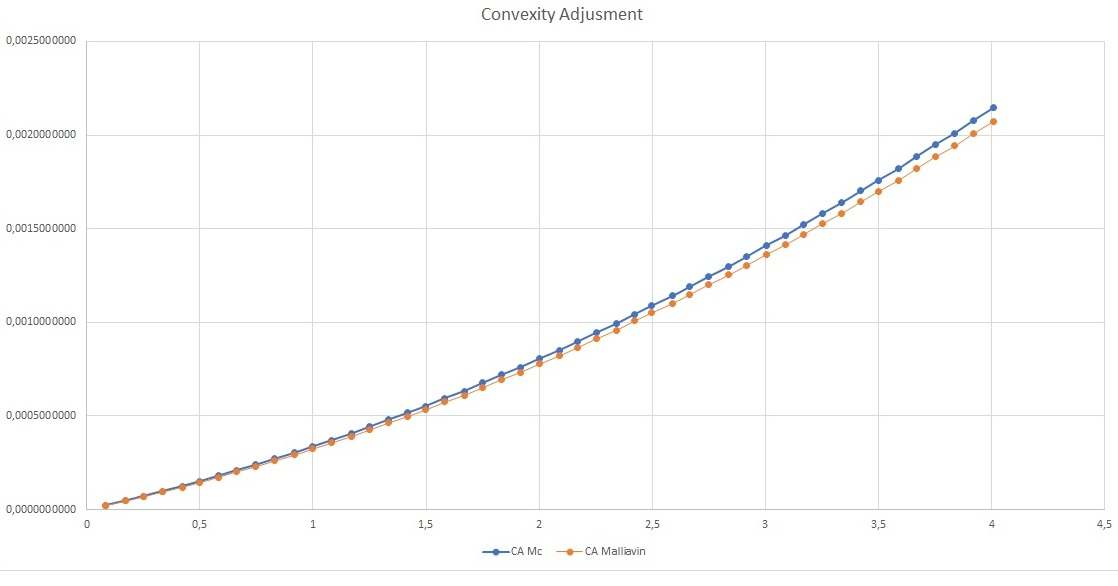
\includegraphics[scale=0.3]{Figures/future_convexity.jpg}
		\caption{Convexity Mc Vs Convexity Malliavin}
	\end{center}
\end{figure} 

\newpage

\subsection{OIS futures}
In this we will derive the covexity adjustment for overnight-indexed swap (OIS) under. We will define for $t_0 < t_1$
\begin{align*}
R(t_0,t_1) &= \frac{\exp\left(\int_{t_0}^{t_1}r_{ois,u} du \right) - 1}{t_1 - t_0} \\
R_{avg}(t_0,t_1) &= \frac{\int_{t_0}^{t_1}r_{ois,u} du}{t_1 - t_0}.
\end{align*}
We must observe, that both $R(\cdot,t_0,t_1)$ and $R_{avg}(\cdot,t_0,t_1)$  are not predictible and they are only observable in $t_1$. However, since
$R(\cdot,t_0,t_1)$ and $R_{avg}(\cdot,t_0,t_1)$ are flows that will be payed in $t_1$, we can considerer the expected value under the measure $\mathbb{Q}^{t_1}$ that will observable during whole period $[t_0, t_1]$. Let us define the next $\mathbb{Q}^{t_1}$ martingales  
\begin{align*} 
\bar{R}(t,t_0,t_1) &= \mathbb{E}^{\mathbb{Q}}\left( R(t_0,t_1)  \right) \\
\bar{R}_{avg}(t,t_0,t_1) &= \mathbb{E}^{\mathbb{Q}}\left( R_{avg}(t_0,t_1)  \right).
\end{align*}
We must do several obeservations. The first observation is that
\begin{align*}
F(t,t_0,t_1)=\mathbb{E}_{t}^{\mathbb{Q}}\left(\exp\left(-\int_{t}^{t_0} r_{ois,u} du \right) R(t_0,t_1) \right) &= \frac{\frac{P_{ois}(t,t_0)}{P_{ois}(t,t_1)} - 1}{t_1 - t_0}, \quad t \in [0,t_0] \\
F(t,t_0,t_1)=\mathbb{E}_{t}^{\mathbb{Q}}\left(\exp\left(-\int_{t}^{t_0} r_{ois,u} du \right) R(t_0,t_1) \right) &= \frac{1}{t_1 - t_0} \left(\frac{\left( \exp\left(\int_{t}^{t_1}r_{ois,u} du\right)\right)}{P_{ois}(t_0,t)}-1\right), \quad  t \in  [t_0, t_1].
\end{align*}
The can define the convexity adjustment for $ R(t_0,t_1)$ the next way
\begin{equation}\label{R_ois_ca}
CA_{ois}(t,t_0,t_1) = F(t,t_0,t_1) - \bar{R}(t,t_0,t_1) 
\end{equation}
The second observation, is that under the dyam we must do is that
\begin{equation}\label{R_ois_avg}
\mathbb{E}_{t}^{\mathbb{Q}}\left(R_{avg}(t_0,t_1) \right) = \mathbb{E}_t^{\mathbb{Q}}\left( \frac{\log\left(1+ \delta_{t_0,t_1} R(t_0,t_1) \right)}{\delta_{t_0,t_1}} \right)  
\end{equation}
In order to compute $\mathbb{E}^{\mathbb{Q}}\left(R(t_0,t_1\right)$, we will define
\begin{equation*}
I(t_0,t_1) = \int_{t_0}^{t_1} r_s ds
\end{equation*}
then for $t < t_0$ from (\ref{clark-okone}) and (\ref{malliavin_derive_x}), we have the next representation for $I(t_0,t_1)$
\begin{align}\label{apprx_I_t0_t1}
I(t_0,t_1) &= \mathbb{E}^{\mathbb{Q}}\left(I(t_0,t_1)\right) + \int_{0}^{t_1}\int_{\max(s, t_{0})}^{t_1}  \mathbb{E}_s^{\mathbb{Q}}\left(\beta(s,u,x_s,y_s) M(s,u) \right) du dW_s^{\mathbb{Q}} \nonumber \\
&\approx \mathbb{E}^{\mathbb{Q}}\left(I(t_0,t_1)\right) + \int_{0}^{t_1}\int_{\max(s, t_{0})}^{t_1} \beta(s,u,x_0,\hat{y}_s) du dW_s^{\mathbb{Q}}\nonumber \\
&= \mathbb{E}^{\mathbb{Q}}\left(I(t_0,t_1)\right) + \int_{0}^{t_1} g(s)h(s,x_0,\hat{y}_s)\int_{\max(s, t_{0})}^{t_1} \exp\left( -\int_{s}^{u} k_{s^{\prime}} ds^{\prime}\right) du dW_s^{\mathbb{Q}}.
\end{align}
Therefore, we can get the next approximation
\begin{align*}
1 + \delta_{t_0,t_1}\mathbb{E}^{\mathbb{Q}^{t_1}}\left(R(t_0,t_1)\right) &= \mathbb{E}^{\mathbb{Q}^{t_1}}\left( \exp(I(t_0,t_1)) \right)\\
&= \exp\left(\mathbb{E}^{\mathbb{Q}}\left(I(t_0,t_1)\right)\right)  \mathbb{E}^{\mathbb{Q}^{t_1}}\left(\exp\left(\int_{0}^{t_1} \Gamma(s,t_0,t_1)dW_s^{\mathbb{Q}}\right)\right)
\end{align*}
where $\Gamma(s,t_0,t_1)= g(s)h(s,x_0,\hat{y}_s)\int_{\max(s, t_{0})}^{t_1} \exp\left( -\int_{s}^{u} k_{s^{\prime}} ds^{\prime}\right)du$. Now, from the Girsanov's theorem we get that
\begin{equation*}
1 + \delta_{t_0,t_1}\mathbb{E}^{\mathbb{Q}}\left(R(t_0,t_1)\right) \approx \exp\left(\mathbb{E}^{\mathbb{Q}}\left(I(t_0,t_1)\right)\right)\exp\left(\int_{0}^{t_1}\frac{\Gamma^{2}(s,t_0,t_1)}{2} ds\right)
\end{equation*}
Therefore we have that
\begin{equation}\label{convexity_ois_future}
\mathbb{E}^{\mathbb{Q}}\left(R(t_0,t_1)\right) \approx \frac{\exp\left(\mathbb{E}^{\mathbb{Q}}\left(I(t_0,t_1)\right)\right)\exp\left(\int_{0}^{t_1}\frac{\Gamma^{2}(s,t_0,t_1)}{2} ds\right) - 1}{\delta_{t_0,t_1}}
\end{equation}
We must note, that from (\ref{apprx_I_t0_t1}) and (\ref{R_ois_avg}) we can get an approximation for $R_{avg}(t_0,t_1)$
\begin{equation*}
R_{avg}(t_0,t_1) = \frac{\mathbb{E}^{\mathbb{Q}}\left(I(t_0,t_1)\right) }{\delta_{t_0,t_1}} \approx \frac{\log\left(1+\delta_{t_0,t_1}  \mathbb{E}^{\mathbb{Q}}\left(R(t_0,t_1)\right) \right)}{\delta_{t_0,t_1}} + \frac{\int_{0}^{t_1}\Gamma^{2}(s,t_0,t_1) ds}{2\delta_{t_0,t_1}}
\end{equation*}
Therefore, since $\log(1+x)\approx x$ we have that
\begin{equation*}
R_{avg}(t_0,t_1) \approx  \mathbb{E}^{\mathbb{Q}}\left(R(t_0,t_1)\right) + \frac{\int_{0}^{t_1}\Gamma^{2}(s,t_0,t_1) ds}{2\delta_{t_0,t_1}}.
\end{equation*}

\begin{remark}
We must observe that for the case $t_0 < t < t_1$ we can compute the convexity adjusment in a similar way when $t < t_0$, but in this case we have to define
\begin{equation*}
I(t,t_1)=\int_{t}^{t_1} r_s ds
\end{equation*}
and 
\begin{align*}
R(t_0,t_1) &= \frac{\frac{\exp(\int_{t}^{t_1} r_{ois,s} ds )}{P_{ois}(t_0,t)} - 1}{t_1 - t_0} \\
R_{avg}(t_0,t_1) &= \frac{\int_{t_0}^{t} r_{ois,s} ds}{t_1-t_0} +  \frac{\int_{t}^{t_1} r_{ois,s} ds}{t_1-t_0}.   
\end{align*}
\end{remark}

\begin{example}
The same way that in the example (\ref{example_ca_future}), we will suppose a Hull-White model with constan mean reversion $k=0.003$ and volatility $\sigma=0.01$. It is easy to show in the case of the Hull-White model
\begin{align*}
\eta_s &= \sigma \exp(-ks)\\
\beta(s,u, x_0, \hat{y}_s) &= \sigma \exp(-ku) \\
\nu(s,t_1) &= \sigma \frac{\exp(-ks) - \exp(-kt_1)}{k}\\
\Gamma(s,t_0,t_1) &= \frac{\sigma \exp(-ks)}{k}\left(\exp(-k(\max(s,t_0) - s)) - \exp(-k(t_1-s))\right)\\
\mathbb{E}^{\mathbb{Q}}\left(I(t_0,t_1)\right)&=-\log\left(\frac{P_{ois}(0,t_1)}{P_{ois}(0,t_0)}\right) + \frac{\sigma^{2}}{2k^{2}}\left(\delta_{t_0,t_1} - 2 \frac{\exp(-kt_0) - \exp(-kt_1)}{k} + \frac{\exp(-2kt_0) - \exp(-2kt_1)}{k}  \right).
\end{align*}
Therefore we have that
\begin{align*}
\frac{\int_{0}^{t_1} \Gamma^{2}(s,t_0,t_1) ds}{2} &= \frac{\sigma^{2}}{2k^{2}} \int_{0}^{t_1}  \exp(-2ks)\left(\exp(-k(\max(s,t_0) - s)) - \exp(-k(t_1 - s))\right)^{2} ds \\
&= \frac{\sigma^{2}}{2k^{2}} \int_{0}^{t_0} \exp(-2ks)\left(\exp(-k(t_0 - s)) - \exp(-k(t_1 - s))\right)^{2} ds\\
&+ \frac{\sigma^{2}}{2k^{2}} \int_{t_0}^{t_1} \exp(-2ks)\left(1 - \exp(-k\delta_{t_0,t_1})\right)^{2} ds\\
&= \frac{\sigma^{2}}{2k^{2}} \left(\delta_{t_0,t_1} \exp(-kt_0) + \exp(-2kt_1) \frac{\exp(-2kt_0)- \exp(-2kt_1)}{2k}\right)\\  
&- \frac{\sigma^{2}}{k^{2}} \frac{\exp(-k(t_1-t_0))- \exp(-k(t_1+t_0))}{k}   \\
&+ \frac{\sigma^{2}}{2k^{2}} \left(1 - \exp(-k\delta_{t_0,t_1})\right)^{2} \left(\frac{\exp(-2kt_0) - \exp(-2kt_1)}{2k}\right)
\end{align*}
Then if we substitute the last equality in (\ref{convexity_ois_future}) we get the convexity adjustment for OIS future. The next figure, show accuracy of (\ref{convexity_ois_future}) in the case of Hull-White


\begin{figure}[h]
	\begin{center}
		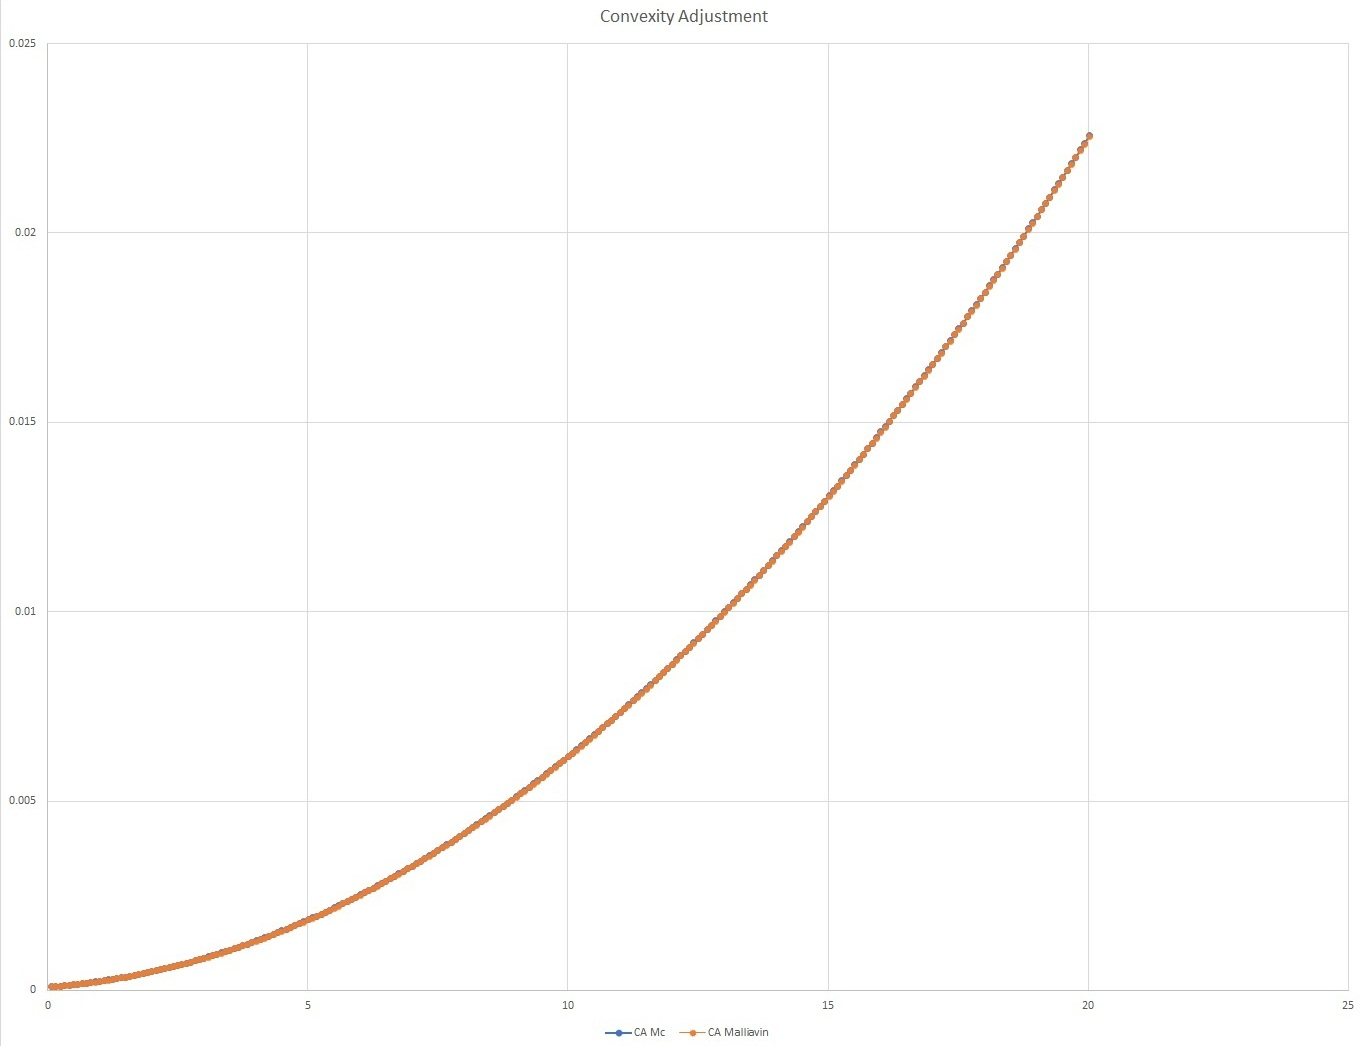
\includegraphics[scale=0.3]{Figures/convexity_ois.jpg}
		\caption{Convexity Mc Vs Convexity Malliavin}
	\end{center}
\end{figure} 

 
\end{example}



\subsection{FRAs in arrears}
The cash flows associated to a FRAs in arrears is $L_{E}(t_1,t_1,t_2)$ in $t_1$. Therefore the payment will be
\begin{equation}
P_{E}(0,t_1)\mathbb{E}^{\mathbb{Q}^{t_1}}\left( L_{E}(t_1,t_1,t_2\right).
\end{equation}
The expected value is clearly taken with respect to the wrong martingale, because $L_{E}(t,t_1,t_2)$ is martingale under the measure $\mathbb{Q}^{t_2}$. In order to calculate, the convexity adjustment we will use as before Clark-Ocone to get a representation for $L_{E}(t_1,t_1,t_2)$ i.e
\begin{equation}\label{general_convexity_fras}
L_{E}(t_1,t_1,t_2) = \mathbb{E}^{\mathbb{Q}^{t_2}}\left(L_{E}(t_1,t_1,t_2) \right) + \int_{0}^{t_1} \mathbb{E}^{\mathbb{Q}^{t_2}}\left(D_s L_{E}(t_1,t_1,t_2) \right) dW^{\mathbb{Q}^{t_2}}_{s}
\end{equation}
The if we suppose the HJM dynamic (\ref{estimation_forward_rate_curve})and we take $\mathbb{E}^{^{\mathbb{Q}^{t_1}}}(\cdot)$ we get
\begin{align*}
\mathbb{E}^{\mathbb{Q}^{t_1}}\left(L_{E}(t_1,t_1,t_2) \right) &= L_{E}(0,t_1,t_2) + \mathbb{E}\left( \int_{0}^{t_1} \mathbb{E}^{\mathbb{Q}^{t_2}}\left(D_s L_{E}(t_1,t_1,t_2) \right) dW^{\mathbb{Q}^{t_2}}_{s}\right)\\
&= L_{E}(0,t_1,t_2) + \mathbb{E}\left( \int_{0}^{t_1} \mathbb{E}^{\mathbb{Q}^{t_2}}\left(D_s L_{E}(t_1,t_1,t_2) \right) (\nu(s,t_2)-\nu(s,t_1)) ds \right)
\end{align*}
Where we have used that 
\begin{equation*}
dW^{\mathbb{Q}^{t_2}}_s = dW^{\mathbb{Q}^{t_1}}_s + (\nu(s,t_2) - \nu(s,t_1)) ds 
\end{equation*}
Now from (\ref{malliavin_derive_x}) we have that 
\begin{equation*}
D_s L(t_1,t_1,t_2) = \frac{G(t_1,t_2)}{\delta_{t_1,t_2}P_{E}(t_1,t_2)} D_s x_{t_1} \approx \frac{G(t_1,t_2)}{\delta_{t_1,t_2}P_{E}(0,t_1,t_2)} \beta(s,t_1, x_0, \hat{y}_s)M(s,t_1)
\end{equation*}
Therefore, if we define 
\begin{equation*}
CA(t_0,t_1) = \mathbb{E}^{\mathbb{Q}^{t_1}}\left( L_{E}\left(t_1,t_1,t_2\right)\right) - L_{E}\left(0,t_1,t_2\right)
\end{equation*}
and we use the last approximation and (\ref{general_convexity_fras}), we can get the next approximation for $CA(t_0,t_1)$ 
\hspace{2cm}
\fboxsep1em
\fbox{\parbox{435pt}
{
\begin{equation}\label{ca_approximations_fra_arrears}
CA(t_0,t_1) \approx  \frac{G(t_1,t_2)}{\delta_{t_1,t_2}P_{E}(0,t_1,t_2)} \int_{0}^{t_1} \beta(s,t_1, x_0, \hat{y}_s) (\nu(s,t_2) - \nu(s,t_1)) ds.
\end{equation}
}}
\begin{example}
To check how works the last approximation. We will restrict a Hull-White model with mean reversion and volatility constant. We will use are $\sigma=0.1$, $k=0.007$ for our model. The analytical approximation that we get from (\ref{ca_approximation_futures}) is
\begin{equation*}
CA(t_0,t_1) \approx \frac{G(t_1,t_2)}{\delta_{t_1,t_2}P_{E}(0,t_1,t_2)}  \frac{\sigma^{2}}{k} \int_{0}^{t_1} \exp(- k(t_1 + u)) -   \exp(- k(t_2 + u)) du 
\end{equation*}
We have checked the last approximation using MC method to compute the value of a FRA in arrears. We will show the result of the simulation in the next figure

\begin{figure}[h]
	\begin{center}
		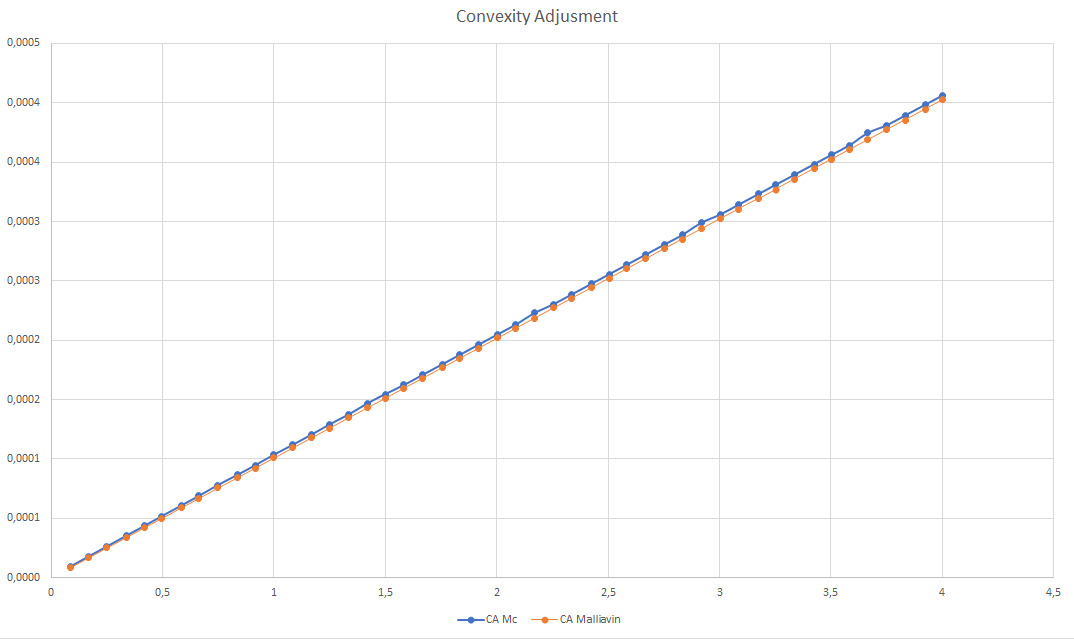
\includegraphics[scale=0.3]{Figures/fra_convexity.jpg}
		\caption{Convexity Mc Vs Convexity Malliavin}
	\end{center}
\end{figure} 
 
\end{example}


\newpage

\subsection{CMSs}

\section{Conclusion}\label{sec:Conclusion}


% TODO: Change bibliographystyle according to the journal style - it should know the online entry, see Matsuda04
\bibliographystyle{spbasic}
\bibliography{references/references,references/references-books,references/references-own,references/references-online}
%\bibliography{references-export}

\end{document}

